\documentclass[12pt,journal]{IEEEtran}
\usepackage[
  backend=biber,
  style=numeric,
  citestyle=numeric
]{biblatex}
\usepackage{graphicx}
\addbibresource{citations.bib}
\providecommand{\keywords}[1]{\textbf{Keywords} #1}
\begin{document}
\title{Traffic Analysis of Large File Downloads on Tor}
\author{\IEEEauthorblockN{William Liddy\IEEEauthorrefmark{1}, Brian Pollack\IEEEauthorrefmark{2}}\\
        \IEEEauthorblockA{Department of Electrical Engineering and Computer Science\\Case Western Reserve University\\Cleveland, OH 44106\\\IEEEauthorrefmark{1}wjl36@case.edu, \IEEEauthorrefmark{2}bmp55@case.edu}}
\maketitle

\begin{abstract}
Tor is a popular anonymity network used by millions to access internet services while maintaining their privacy. The main idea behind Tor is that clients build a "circuit" of relays, where each relay carries traffic to the next relay, without any single relay knowing the full extent of the path. Thus, anonymity is achieved, because no relay can trace the client to the destination. 

However, A paper written in 2005 titled "Low-Cost Traffic Analysis of Tor" by Steven J. Murdoch and George Danezis demonstrated that a traffic analysis attack was possible against the Tor network. Any attacker could monitor the load on a relay in the Tor network by calculating the RTT to the relay, and when the RTT spiked, it was clear that the relay was being used. With this information, attackers could trace the path of a client in the Tor network and de-anonymize them.

This paper was written in 2005, when Tor was still young. At the time of Murdoch and Danezis' paper, the entire Tor network consisted of just fifty relays. As the time of writing, there were well over 7,000 relay relays in the network, so the ecosystem of Tor is radically different. With all of the increased traffic, we wanted to discover if this type of attack was still valid, and would not be masked by other traffic.

Our results indicate that if a victim is downloading a large file as fast as Tor will allow them to, a decrease in bandwidth and an increase in round trip time (RTT) is usually observable on the relay. We also discovered that Tor guard relays, a special subset of relay that clients will pick at the first hop in their circuit, are very susceptible to this kind of attack.

\end{abstract}

% \keywords\\{TOR; Onion Routing, }

\section{Introduction}
\IEEEPARstart{T}{or} 
\section{Background}
\subsection{Tor Architecture}
Tor is a circuit-based anonymous communication service that uses Onion Routing to securely pass packets in the network.
\par
A Tor circuit is the path that communication takes from the client to the desired destination. A circuit consists of multiple servers, called relays, and is typically three hops long. To set up a circuit, the client must know the IP addresses of the three relays of which it would like to build the circuit of. The Tor network provides a list of appropriate relays through a service called a directory authority. The client then can send TCP packets through the circuit.
\par
Onion Routing is an overlay network protocol that is designed to carry TCP packets over a circuit without revealing the path of the circuit to any single relay. To set up an onion-routed circuit, the client starts by encoding the IP address of the destination with the public key of the last relay, then encoding that entire message with the key of the second-to-last relay, and so on. When the first relay receives the packet to transmit, it "unwraps" a layer from the packet using it's private key and forwards the message to the address of the relay that is revealed. The packet is unwrapped like an union, which is where the name comes from.
\par
Tor routes its traffic using Onion Routing. A user will set up a circuit using at least three Tor relays, and that circuit stays active until the user either is finished or requests a new circuit. Tor circuits can carry any TCP packet, as long as the application supports routing through Tor, however, it cannot carry UDP packets. A single Tor circuit can carry multiple simultaneous streams, which is good for HTTP traffic which opens multiple connections to multiple destinations.
\par
One common attack against anonymous communication networks is known as traffic analysis attack. An attacker will analyze the traffic through a network to try to de-anonymize a user. While some anonymity services will reorder, mix, or otherwise shape the traffic flowing between Onion Routers, Tor chooses to not attempt to shape the traffic. The creators believed that all currently available traffic shaping strategies were still vulnerable to attacks and were difficult to implement practically. They also wanted to make Tor as low-latency as possible, and reordering packets would increase latency.
\par
Furthermore, to protect against traffic bottlenecks, Tor uses a decentralized congestion control mechanism that sends end-to-end ACK packets to maintain anonymity while allowing edge relays to detect congestion and throttle their traffic until congestion subsides.
\par
Traffic is only allowed to leave the Tor network through relays which specifically allow exits (called exit relays). Each relay has a policy stating which traffic is allowed to leave the network: this can be restricted by IP address or protocol. \cite{Dingledine:2004:TSO:1251375.1251396}

\subsection{Tor Threat Model}
Tor is designed to be impossible for attackers to link users with the services to which they are connecting \cite{Dingledine:2004:TSO:1251375.1251396}. The main goal of most attackers to the Tor network, therefore, is to de-identify its users and observe the remote services they are accessing. The attacker would then be limited by other encryption protocols, such as HTTPS, but that is beyond the scope of our study. A secondary goal of an attacker would be to group network connections, establishing a link among multiple connections to the same initiator. This would allow the attacker to build a profile on the user be observing with whom the user is communicating and by observing the user's communication habits \cite{Murdoch:2005:LTA:1058433.1059390}.
\par
If an attacker could identify individual users, this would constitute a major problem for Tor. The entire point of Tor is to keep users anonymous, and if it is proven that it is possible to de-anonymize users, then the Tor network has a significant flaw that needs to be addressed.
\par
Tor is designed to protect against an adversary who can observe some fraction of network traffic. This adversary can generate, modify, delete, or delay traffic and can operate his or her own Tor relays. The adversary can also compromise some fraction of existing Tor relays\cite{Dingledine:2004:TSO:1251375.1251396}.
\par
Additionally, it is important to note that Tor does not protect against traffic confirmation attacks, which occur when an adversary suspects two parties are communicating and tries to prove it by analyzing the network. Tor rather attempts to make it difficult to identify who is communicating without a solid suspicion \cite{Murdoch:2005:LTA:1058433.1059390}.
\par
With our attack model, we try to gain information about the path of the Tor circuit using methods available to all Tor users. It is important to note that we do not exit the threat model for which Tor is built. We demonstrate that anyone with sufficient know-how and a few Tor relays can potentially de-anonymize Tor users- no large investment or "insider" information is needed.
\subsection{Tor Traffic Analysis}
Traffic analysis is the process of observing traffic from a network and making assumptions about users based. Metrics these assumptions use include the timing of packets and header information such as source and destination IP addresses. In the scope of anonymous networks, traffic analysis can be used with the goal of identifying end-users who are trying to remain anonymous \cite{Murdoch:2005:LTA:1058433.1059390}.
\par
On the Tor network, traffic analysis cannot be used to read the header information or content of the original TCP packets that are transmitted through the network while the packet is still in the Tor network. This type of traffic analysis can also be performed both before and after the original packet enters and leaves the Tor network, but that is beyond the scope of our threat model.
\par
Traffic analysis can be performed on the packets traveling through the Tor network. The attacker will not be able to read the header information of the original TCP packets because they are encased in the onion routing packets, but an attacker is able to gain information based on those onion routing packets.
\par
The type of traffic attacks which are most dangerous to the Tor network involve observing the traffic on a particular Tor relay. Because Tor does not delay or reorder packets, we believe it to be susceptible to various types of traffic analysis attacks.
\par
Traffic analysis can be performed in multiple ways. An attacker can directly observe packets if he or she controls part of the network. Alternatively, an attacker can indirectly gain insights on a relay by using measurements such as round trip time (RTT) or a measurement of throughput on the relay.
\par
We believe that if an attacker is observing a subset of relays, he or she is able to effectively identify end-users requesting large amounts of bandwidth through traffic analysis. Because we do not require a global observation of the network and do not require many Tor relays under the attacker’s control, our network analysis attack is within the Tor threat model.


\begin{figure*}

 \center
  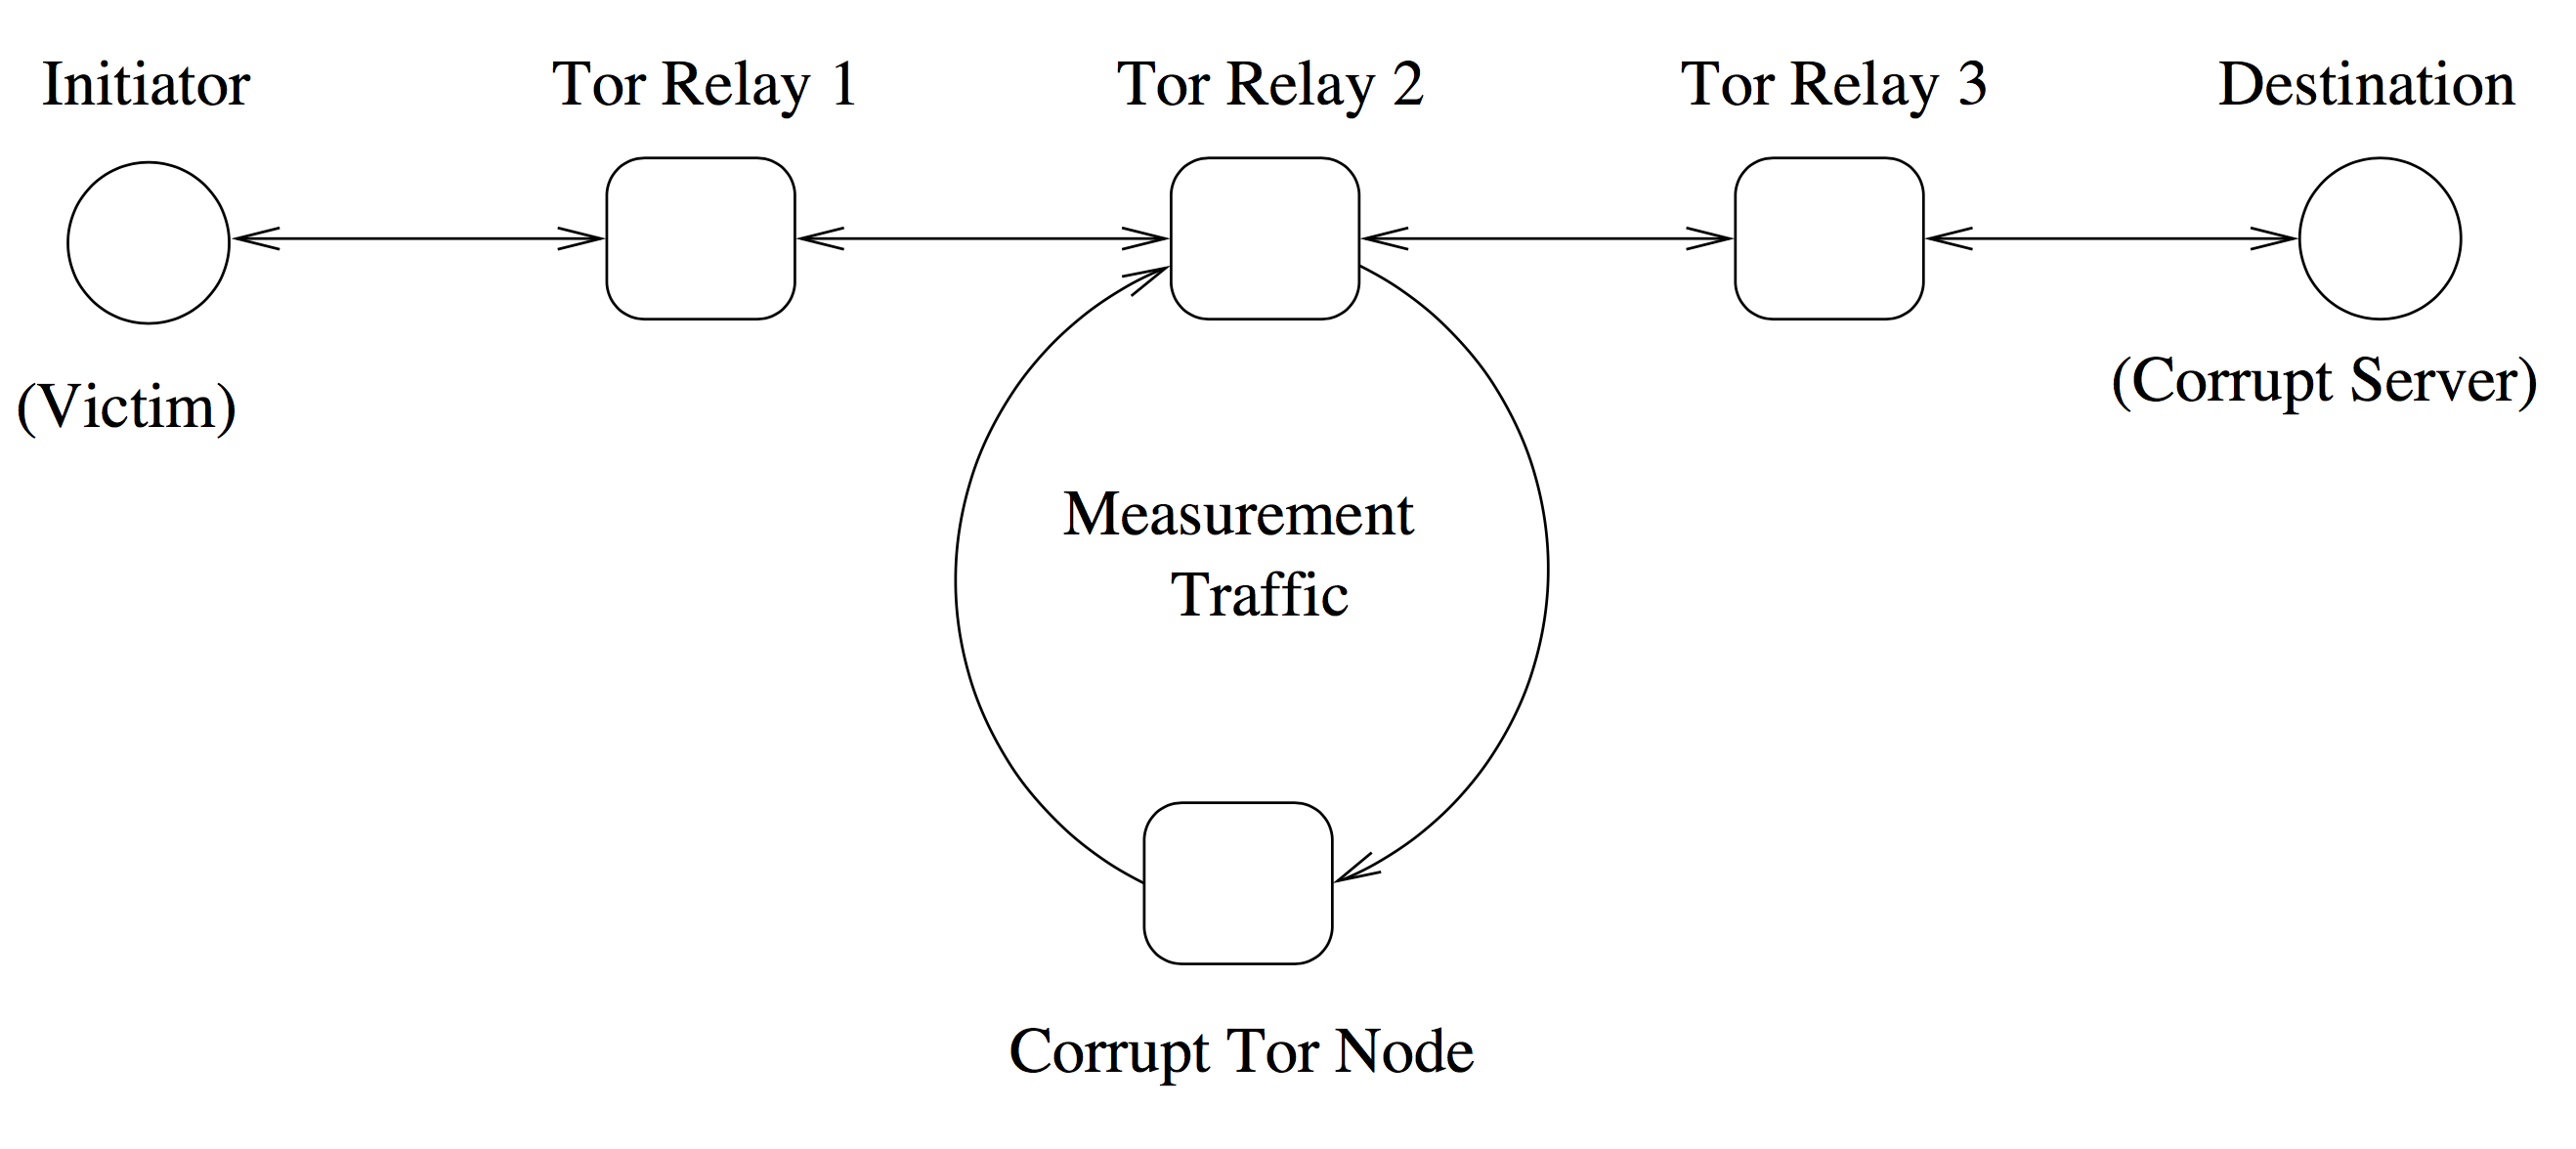
\includegraphics[width=\textwidth]{figures/murdochattacksetup.png}
  \caption{Murdoch and Danezis's Attack Setup \cite{Murdoch:2005:LTA:1058433.1059390}}
  \label{murdochsetup}
\end{figure*}

\subsection{Previous Work}
In 2005, Murdoch and Danezis studied the possibility of network analysis attacks on the Tor network. In their attack model, an adversary created a corrupt Tor relay on the network. The corrupt relay was then used to measure other relays' traffic load by measuring the RTT to that relay. Additionally, they assumed that the attacker controlled a network server that the victim is accessing. Murdoch and Danezis claim that this threat is within the threat model that should be covered by Tor. If the attackers modulate the data through the network server that the user is accessing, they were able to observe similar modulations in the Tor circuit that the user was using. This means, therefore, that the attackers could trace the user through the Tor circuit and link a user with the services he or she is using \cite{Murdoch:2005:LTA:1058433.1059390}. Figure \ref{murdochsetup} shows Murdoch and Danezis's attack setup.
\par
Because Murdoch and Danezis were able to observe the change in traffic patterns as users connected to a web service through a Tor circuit, they could infer which relays were part of that circuit. This information alone, however, does not seem to be useful. The attacker may have identified servers through which a victim communicated, but have not yet found that victim. If the attacker has access to the user's ISP, then the attacker can get the logs of the IP is communicating with the discovered relays in the Tor circuit and therefore can most likely identify the exact user who is trying to remain anonymous. This makes Tor insecure for users who have ISPs that are not willing to protect their privacy, such as countries where government controls the ISP in order to censor material.
\section{Our Setup and Results}
We wanted to test if the modern Tor network was still vulnerable to Murdoch and Danezis's attack, given that the popularity of Tor might mask traffic, making analysis impossible. But we did not duplicate the attack exactly- rather, we modified it slightly and reevaluated the exact attack scenarios. Our attack specifically targets "guard relays", which are the first relays in every Tor circuit.
\subsection{Consensus Values}
When a Tor relay is first created, it goes through four phases as it is being added to the Tor network. Each phase allows a different amount of traffic to be routed through the new relay.
\subsubsection{Consensus Weight}
If anybody could immediately add a relay to the Tor network and advertise that it can handle a large amount of traffic, other users would immediately start sending data through that new relay. This means that an adversary could easily set up a relay and allow many clients to set up circuits through it, then delay or drop those connections. It would be easy for adversaries to disrupt the Tor network. To combat this issue, Tor assigns a measurement to each relay called consensus weight. Each client starts with a low consensus weight and, as other users send data through the new relay, if the Tor network determines that the new relay is performing well, the consensus weight will increase. The Tor network sends more traffic to relays with a higher consensus weight.
\subsubsection{Guard relays}
On the Tor network, most clients build three hop circuits. The very first Tor relay with which a client interacts is slightly different than the rest because it helps protect the client against certain attacks. This first relay is called a guard relay. An anonymity attack that may be performed on the Tor network can look like this: if a client picks N paths at random, and an adversary controls a few Tor relays, then over time the chance that the client has made no connections through compromised Tor relays goes to zero. The philosophy behind guard relays is that the client will pick a guard relay and will make every subsequent Tor circuit using that same guard relay as the first hop. Either all of the client's connections will be compromised (the guard relay will know the IP address of the client), or none of the client's connections will be compromised (each subsequent relay in the circuit may know the guard relay, but will never know the IP of the client). Once a Tor relay is listed as a guard relay, most clients will not use it as a middle relay in a Tor circuit. This helps prevent the few relays which are trusted as guard relays from being overloaded \cite{arma2013}.
\subsubsection{Phase 1: unmeasured}
When a relay is first started, it will self-test its bandwidth. It publishes the results to its relay descriptor. For the first few days, the Tor network will allow only 20KB/s of bandwidth through the new relay \cite{arma2013}.
\subsubsection{Phase 2: remote measurement}
After a few days, the new relay will have received enough connections, despite its bandwidth being capped at 20KB/s, to begin to receive an increased consensus weight. When more traffic is received, if the relay performs well enough, the consensus weight will be raised even more. During this phase, however, a relay cannot be a guard relay. The relay will remain a middle relay in the Tor network until moving on to phase three \cite{arma2013}.
\subsubsection{Phase 3: ramping up, guard relay}
To become a guard relay, a relay must have a large enough consensus weight, a high enough uptime percentage, and a long enough time known to the Tor network. A relay is eligible to become a guard relay on the eighth day of its existence on the Tor network, assuming the first two conditions are satisfied. Over time, more and more clients will use the new relay as a guard relay and will remember that relay to use for their next connections \cite{arma2013}.
\subsubsection{Phase 4: steady state, guard relay}
Finally, once the new Tor relay has been a guard relay for approximately twelve weeks, it will reach a steady state in which the number of new clients connecting to it as a guard relay is equal to the number of clients who decide to choose a new guard relay. This prevents the oldest guard relays from becoming overloaded with traffic \cite{arma2013}.
\subsection{TORRC Configuration}
To configure the Tor service, the relay operator has to modify the torrc configuration file. We would like to point out that a relay operator may choose to force the relay to use a smaller bandwidth than his or her network will allow. An operator may choose to restrict bandwidth for a variety of reasons.
\par
It is also worth stating that there are many other configuration options for the Tor service, and they are mostly located in the torrc configuration file. An operator can choose whether or not to allow the relay to operate as a relay relay or as an exit relay and can set the ports that the Tor service uses, among many other configuration options.
\subsection{Our Attack}
\begin{figure*}
 \center
  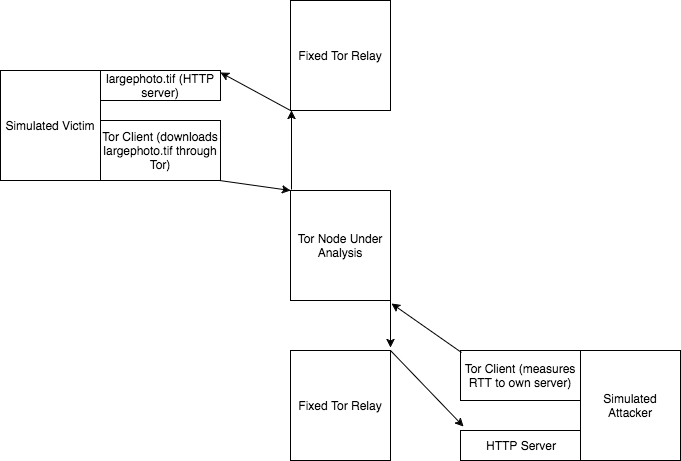
\includegraphics[width=\textwidth]{figures/oursetup.png}
  \caption{Our attack setup}
  \label{oursetup}
\end{figure*}
\subsubsection{Our Threat Model}
We begin with the assumption that a client will be accessing a service over the Tor network (in our case, an HTTP server). We also assume that an attacker has some control over and can generate, modify, delete, or delay traffic on either the client's network or the network of the web service. Lastly, we assume that the attacker has the ability to add a few relays to the Tor network. All three of these assumptions are within the Tor threat model \cite{Dingledine:2004:TSO:1251375.1251396}.
To simulate the attacker, we first set up one Tor relay and one Tor exit relay, both using Lightsail on Amazon Web Services, and waited for them to be accepted to the Tor network.


\subsubsection{Our Victim}We then set up a simulated victim machine which used the Tor network to download a large (1 GB) photo. The photo was hosted on an Apache Webserver on the same machine as the victim. The reason the victim routed to itself was to assure that the Tor network was the bottleneck- not our Webserver. Additionally, using a public resource might throttle the client or otherwise cause changes in bandwidth during the experiment, which would lead to undesired modulation in the data due to the change the traffic going through the Tor network. The victim client used the Tor network to reach a fixed exit relay which would then connect back to the Webserver and download the image.
\par
The victim client was programmed accept a list of Tor relay addresses. With this list, the victim client would construct a 2-hop Tor circuit that consisted of the first relay in the list, then the fixed exit relay. The victim would then proceed to download the image for sixty seconds, then pause for sixty seconds, then repeat this process with the next relay in the list. This list was also sent to the analysis relay, which is covered in the next section.

\begin{figure*}
 \center
  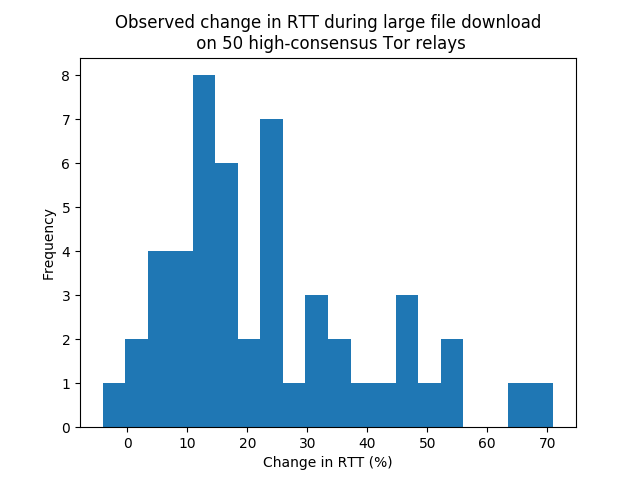
\includegraphics[width=0.4\textwidth]{figures/rtt_guard.png}
  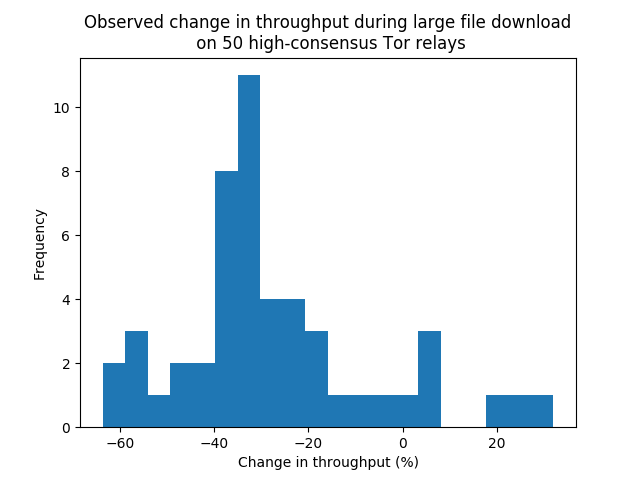
\includegraphics[width=0.4\textwidth]{figures/thr_guard.png}
  \caption{Results of run over 50 high-consensus relays}
  \label{AAA}
\end{figure*}

\begin{figure*}
 \center
  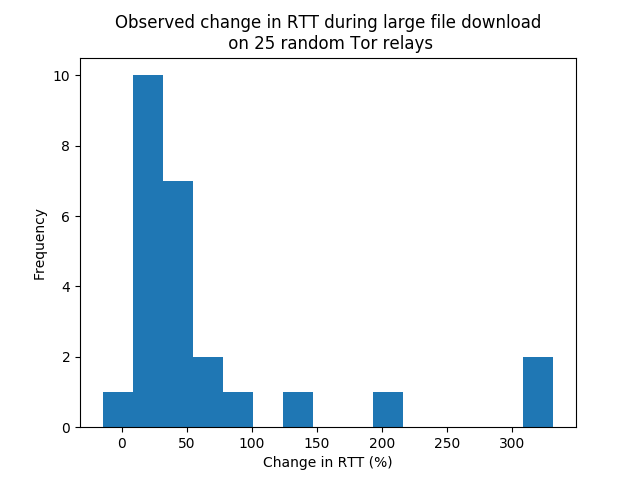
\includegraphics[width=0.4\textwidth]{figures/rtt_avg.png}
  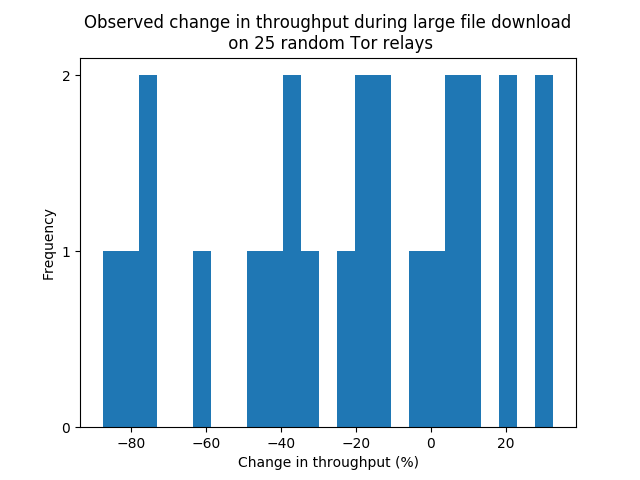
\includegraphics[width=0.4\textwidth]{figures/thr_avg.png}
  \caption{Results of run over 25 random relays. Outliers excluded.}
  \label{AAA}
\end{figure*}

\subsubsection{The Analysis Exit relay} The Analysis exit relay has the same list of relays as the victim, and since the victim is deterministic in it's timing, the analysis relay knows exactly what relay the victim is connected to. The analysis relay sets up a Tor circuit through the relay the victim is currently connected to. It would measure both the change in RTT and change in throughput (via downloading a large file, with the same setup as the client) through the analyzed relay during and after the download. See figure \ref{oursetup} for a diagram of our setup.

\subsubsection{Implications}
This setup is not unreasonable. We had three machines involved, including both the victim and analysis relays. If the attacker has access to a victim's network, he or she could modulate the traffic by delaying packets, causing similar delays that we were using to experiment. If the attacker has access to the server to which the victim is connecting, the attacker can modulate the traffic there.
One additional way, which is the easiest for attackers to exploit, is for an attacker to interject his or her own content into the victim's connection by serving his or her modulated content on a legitimate website that the victim is accessing. For example, the simplest way of forcing the victim to download this modulated traffic is if the attacker purchased an advertisement on a website the victim was browsing. The attacker could then modulate the content that is downloaded by the client to load the advertisement.
Next, the attacker would need to have enough analysis relays to be able to measure a significant percentage of the available Tor relays. Because the attacker does not know any information about the victim's Tor circuit, he or she will need to analyze multiple relays until the circuit is discovered. Especially if the search was limited to a subset of the active Tor relays, we believe it is not unreasonable to assume that this attack is possible. The subset of measured relays could start with all of the guard relays, for example, which we know should constitute one hop in the victim's circuit.
\par
It should also be noted that in our attack model, we assume the client is downloading a file from Tor as quickly as Tor will allow them to. While this is the same technique that Murdoch's attack uses, it should be noted that traffic analysis attacks such as this one are limited to situations where the victim is obtaining a large amount of data over a long period of time. We acknowledge that this attack will not work against users requesting resources sporadically- such as just viewing HTML pages, and reading them. This attack is still very valid against victims who are downloading a large file or streaming content.



\subsection{Our Results}
Firstly, we ran our analysis on the 50 highest-consensus relays in the network. These were made publicly available through a service called Onionoo. The results of the RTT analysis and bandwidth analysis are shown in figure 3.
\par
When the victim was downloading a file through one of these relays, the observable RTT increased by 23.5\% compared to when the victim was not downloading anything, on average. Of the 50 relays tested, an increase in RTT was observable on 49. This means that for an overwhelming majority of high-consensus relays (those likely to be guard relays), traffic analysis attacks are still very possible given that the victim is using a lot of bandwidth.
\par
We also expand on Murdoch's findings by introducing the idea that throughput analysis attacks are viable. When the client was downloading a file through one of these relays, the observable throughput when another Tor user was also downloading a file decreased by 27.2\% compared to when the victim was not downloading anything, on average. Of the 50 relays tested, an decrease in throughput was observable on 43 of the relays. While not as sure-fire as the RTT for traffic analysis, most relays are still susceptible to this kind of analysis.

\par
We also ran our analysis on 50 randomly selected relays from the Tor network. Many of these relays acted erratically, and we would regularly see connections dropped, and RTTs and throughput go to zero in the middle of a run. Of the 33 relays that had successful runs, we removed the 4 highest and 4 lowest outliers for a total of 25 relays. This is shown in figure 4.
\par
When the victim was downloading a file through one of these relays, the observable RTT increased by 65.4\% compared to when the victim was not downloading anything, on average. Of the 25 relays tested, an increase in RTT was observable on 24.
\par
When the victim was downloading a file through one of these relays, the observable throughput when another Tor user was also downloading a file decreased by 20.2\% compared to when the victim was not downloading anything, on average. Of the 25 relays tested, an decrease in throughput was observable on 18 of the relays.
\par
While 25 relays is hardly a sufficient sample size for a population of 7,000, it does hint that RTT is a better measure for relays in general, rather than throughput analysis.

\section{Conclusions}
We have demonstrated that traffic analysis attacks using RTT as described by Murdoch are still effective, given that the client is downloading a large file using all possible resources available to him or her. We also introduce the idea that throughput analysis attacks are possible.
\par
Given that this attack is demonstrated to only work on victims who are generating a large amount of traffic, the next step is to figure out what bandwidth users can reasonably make use of when downloading or streaming content over Tor without risk of de-anonymization. Tor relays must make sure that, even under load, the RTT and bandwidth available remains constant.
\printbibliography
\end{document}
